\documentclass[12pt]{article}
\usepackage{geometry}                % See geometry.pdf to learn the layout options. There are lots.
\geometry{letterpaper}                   % ... or a4paper or a5paper or ... 
%\geometry{landscape}                % Activate for for rotated page geometry
\usepackage[parfill]{parskip}    % Activate to begin paragraphs with an empty line rather than an indent
\usepackage{daves,fancyhdr,natbib,graphicx,dcolumn,amsmath,lastpage,url}
\usepackage{amsmath,amssymb,epstopdf,longtable}
\usepackage[final]{pdfpages}
\DeclareGraphicsRule{.tif}{png}{.png}{`convert #1 `dirname #1`/`basename #1 .tif`.png}
\pagestyle{fancy}
\lhead{CE 3354 Engineering Hydrology}
\rhead{FALL 2024}
\lfoot{}
\cfoot{}
\rfoot{Page \thepage\ of \pageref{LastPage}}
\renewcommand\headrulewidth{0pt}



\begin{document}
\section*{Syllabus}

%%%%%% BEGIN SYLLABUS COMPONENT %%%%%%%%%%%%%%%%%%%%%%%%%%%%%%%%%%%%%2010-0814TGC%%%%%%%%%%%%%%%%%%%%%%%%%%%%%%%%%%%%%%%%%
\subsection*{{Course Location, Textbook, Instructor Contact Information}}
\begin{tabular}{p{1.5in}p{5.0in}}
Class meetings: &   2:00-3:20PM, T-TH, IE205 (Section 001) \\
Instructor: & Theodore G. Cleveland, CE Room 203F \\
TA: & none \\
Office Hours: & TBD \\%P. Monaco MW 13:00-15:00 \\
%~ & T. Cleveland MW 08:00 - 10:00 \\
Telephone: & (806)834-5101 \\
Cell Phone: & (832)722-4185 (more reliable than office phone) \\
E-mail: & \texttt{theodore.cleveland@ttu.edu}\\
Web: & \texttt{http://54.243.252.9/ce-3354-webroot}\\
%%%%%%2010-0814TGC%%%%%%%%%%%%%%%%%%%%%%%%%%%%%%%%%%%%%%%%%
Textbook(s) : & \cite{CMM1988} (Copy on Server) \\
~ & \cite{Dooge1973} (Copy on Server) \\
~ & \cite{McCuen2002} (Copy on Server) \\
~ & \cite{Viessman1977} (Copy on Server) \\
 %\cite{cleveland2013} \\
 %%%%%%2010-0814TGC%%%%%%%%%%%%%%%%%%%%%%%%%%%%%%%%%%%%%%%%%
Copyright : & \textsl{Copyright $\copyright$ 2014 Theodore G. Cleveland, all rights reserved.} \\
\end{tabular}
%%%%%%2010-0814TGC%%%%%%%%%%%%%%%%%%%%%%%%%%%%%%%%%%%%%%%%%
\subsection*{{Catalog Description}}
\begin{quote} \textbf{3354. Engineering Hydrology (3:3:0).}  Prerequisite: CE 3305. Analysis and design methods related to the occurrence and distribution of surface and groundwater; precipitation, infiltration, runoff, and frequency analysis. (Writing Intensive)
\end{quote}
%%%%%%2010-0814TGC%%%%%%%%%%%%%%%%%%%%%%%%%%%%%%%%%%%%%%%%%
%%%%%%%%%%%%%%%%%%%%%%%%%%%%%%%%%%%%%%%%%%%%%%%%%%%%%%%
%%%%%%%%%%%%%%%%%%%%%%%%%%%%%%%%%%%%%%%%%%%%%%%%%%%%%%%
\subsection*{{Course Objectives}}
The purpose of this class is to study the theory and application of hydrologic concepts; learn how to use predictive tools such as charts and computer programs, and apply these tools to the analysis and design of collection and drainage systems.  Preparation of professional reports is a substantial component of this course.
\subsubsection*{{Knowledge, Skills, Abilities (KSA)}}
During this course the student will
\begin{enumerate}
\item Read, synthesize, and communicate ideas presented in current and historical technical literature.
\item Delineate watersheds from maps and determine common metrics (area, slope, main channel length) using digital planimetry.
\item Perform hydrologic computations using Excel, as needed\footnote{This task is principally to develop understanding of how the professional tools function.  Excel is a professional tool in its own right, but the skill level to use for engineering is beyond the scope of this class.}.
\item Perform hydrologic simulation using HEC-HMS.
\item Size and select engineering materials (pipes) for use in drainage engineering.
\item Prepare professional reports for the design of a stormwater management system.  

\end{enumerate}

\subsection*{ABET Program Outcomes}
A subset of the ABET Program Outcomes are addressed in CE 3354, these outcomes are listed below:\footnote{Item 3[b] below is only partially fulfilled --- in this course students will analyze and interpret data, design of experiments is beyond the scope of the class.}


\begin{tabular}{p{0.5in}p{5.5in}}
\texttt{3[a].}  & Ability to apply knowledge of mathematics, science, and engineering.\\
\texttt{3[b].}  & Ability to design and conduct experiments, as well as to analyze and interpret data.\\
\texttt{3[c].}  & Ability to design a system, component, or process to meet desired needs.\\
\texttt{3[e].}  & Ability to identify, formulate, and solve engineering problems.\\
\texttt{3[i].}   & Recognition of need for life-long learning.\\
\texttt{3[k].}  & Ability to use the techniques, skills, and modern engineering tools necessary for engineering practice.\\
\texttt{8[e].}  & (Civil Engineering) Proficiency in water resources engineering. \\
\texttt{8[a].} & (Environmental Engineering) Proficiency in mathematics through differential
equations, probability and statistics, calculus-based physics, general chemistry, an earth
science, e.g., geology, meteorology, soil science, relevant to the program of study, a biological
science, e.g., microbiology, aquatic biology, toxicology relevant to the program of study, and
fluid mechanics relevant to the program of study. \\
\texttt{8[d].} & (Environmental Engineering) Ability to perform engineering design by means of
design experiences integrated throughout the professional component of the curriculum. \\
\texttt{8[f].} & (Environmental Engineering) Data acquisition for hydrologic design is explained and
the role of certain organizations in providing information and guidance is emphasized. \\
\end{tabular}
%\newpage

%==========STANDARD COURSE POLICY MATERIALS, SHOULD NOT CHANGE OFTEN=======
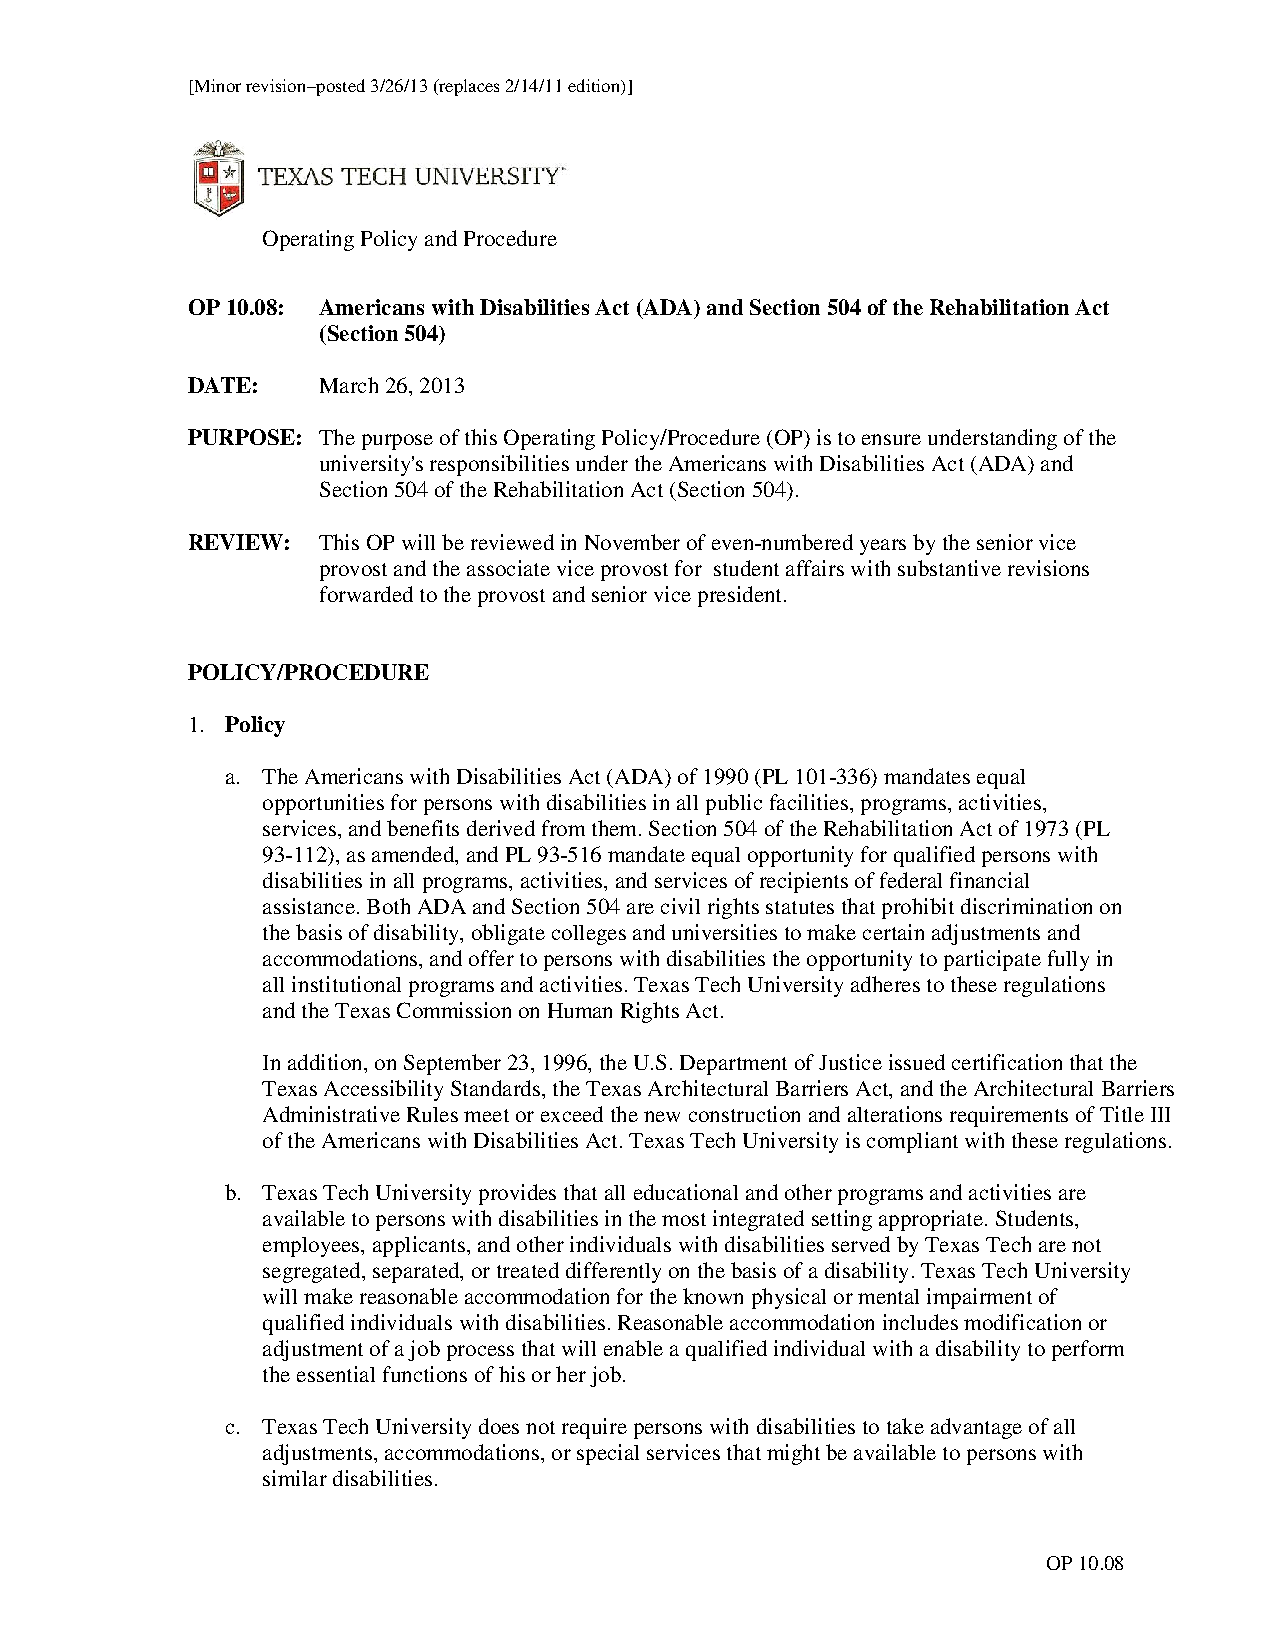
\includepdf[pages=-]{./OP10-08.pdf}

\section*{Course Specific Policies}
\subsection*{Disability:}
Texas Tech policy provided as part of syllabus (see preceding section).

\subsection*{Religious Holidays:}
\textsl{ "A student who intends to observe a religious holy day (as defined by OP 34.19) should
make that intention known to the instructor prior to the absence in order to receive accommodations
prescribed by OP 34.19."}

\subsection*{Cellphones/Pagers: }
Please set your personal communication devices to silent ring or off during class. 
Do not take calls in class. Disturbance during class time is not acceptable.

\subsection*{Prerequisites:} 
Mastery of material from CE 3305 or equivalent is expected.

\subsection*{Attendance:} Roll will be taken to determine attendance for class participation.  Please let the instructor know in advance if you must miss a class for a legitimate reason\footnote{Legitimate reasons include: Academically-related extracurricular activities (ASCE, AGU, etc.); Illness with documentation; Federal Family Leave Act Policies; Orders to activate (Military, Peace Officer, Public Health, etc.).  Bring me some kind of documentation for such absences.}. 

\section*{Evaluation Instruments and Grading}
Student performance will be evaluated using attendance (coming to class), exercises (homework), project reports, and examinations.   The exams will derive much of their content from the exercises.  At the end of the semester students are to turn in a portfolio of all graded work.  The portfolio should be comprised of photocopies of exercise materials, and exams 1 and 2.  The project report should be submitted under separate cover.  The portfolio should be bound using a binder clip.  The portfolio will not be returned.  

%\subsection*{Article Reviews:} 
%Several article reviews are assigned; part of professional development is reading and interpreting professional literature.  Due dates for these reviews are shown in Table \ref{tab:fall2014schedule}.  These reviews are shown as \texttt{R-\#}.

\subsection*{Exercises:} 
Team assignments will be assigned during the semester.  
These exercises will be graded on a ten point criteria\footnote{Legibility, correct method, and correct answer are components of the criteria.   The grader will not diagnose sources of arithmetic or algebra errors unless the errors are obvious.  Solutions are presented in class and posted on the server }.
\begin{enumerate}
\item Every homework assignment is to be accompanied by a descriptive report containing your analysis
of the problem. Report materials should be prepared with a word processor. 
Hand computations may be turned in on engineering paper; important steps in each solution must be shown for credit. 
Legibility is determined by the grader; illegible materials will receive no credit.
\item Assignments are due at the beginning of class. Late assignments are not accepted.  Be sure the team number and team members are on each page.
\item Due dates are shown in Table \ref{tab:fall2013schedule};  Exercises are denoted by \texttt{ES-\#}
\end{enumerate}

\subsection*{Engineering Report:}  
A project report comprised of various components developed during the course is to be completed.  The project is introduced early in the semester and is related to the hydrologic analysis of a watershed.   A draft report is due and shown as \texttt{RP-1}.   This report will be critiqued and suggestions for the final report provided.   An intermediate report is due and shown as \texttt{RP-2}.  The final report, incorporating the suggestions is due at the last class meeting and is shown as \texttt{RP-3}.

\subsection*{Exams:} Three examinations will be given, they will be of approximately equal difficulty.
\begin{enumerate}
\item Examinations are open notes.
\item Examinations are comprehensive, even though the main focus will be the materials discussed prior to the examination.
\item Full credit for problems will only be given if all computations are documented.
\item Examination dates are shown in Table \ref{tab:fall2013schedule}.
\end{enumerate}

\section*{Grading:} Final grades are determined based on performance during the semester.  Letter grades will be assigned using University standards.  The \textbf{approximate} weighting of graded material in determining the final grade is as follows\footnote{Graded materials with fewer than 100 points will have raw scores reported and will be normalized to 100 points for calculating the final grade.}:
% Requires the booktabs if the memoir class is not being used
\begin{table}[h!]
   \centering
   \begin{tabular}{l l}
Item & Percent of Grade \\
\hline
\hline
Attendance & 10\% \\
Exercises & 20\% \\
Project Report & 20\% \\
Examinations & 50\% \\
\hline
\end{tabular}
\end{table}

\textbf{Cheating:} Dont.

%%%%%%%%%SCHEDULE GOES HERE %%%%%%%%%
%%%%%%%%% Use Comment to Maintain History %%%%%
\clearpage
\section*{Schedule}
\begin{table}[ht!]
   \centering
   \caption{Spring 2016 Course Schedule}
   \begin{tabular}{p{0.5in}p{3in}p{2.5in}} 
   ~ & ~ & ~  \\
\hline
\hline
DATE & TOPIC & READINGS  \\
\hline
\texttt{22AUG24} & Introduction &   \\ %0
\texttt{27AUG24} & Specialized Software &  \\ %1 
\texttt{29AUG24} & Hydrologic Cycle  &  \\ %2 water budget(s)
\texttt{~3SEP24} & Hydrologic Data Sources &\\ %3 streamflow measurement, precipitation measurement, online archives
\texttt{~5SEP24} & Watersheds and GIS &  \\ %4 watershed definitions and delineation, metrics of interest
\texttt{10SEP24} & Probability Estimation Modeling &  \\ %5
\texttt{12SEP24} & Streamflow and Hydrographs &  \\ %6
\texttt{17SEP24} & WCOE Job Fair (Civil Engineering)   &   \\ %7
\texttt{19SEP24} & Floods and Flood Frequency Analysis &  \\ %8
\texttt{24SEP24} & Precipitation, Hyetographs, Design Storms &   \\  %9 NOAA Atlas 14, PFDS, Create design storm
\texttt{26SEP24} & \textbf{Exam 1} &  \\ % XBS Watershed Delineation; Flood Frequency; Water Budget; 
\texttt{~1OCT24} & Evaporation and Infiltration Losses &  \\ %10
\texttt{~3OCT24} & Rainfall-Runoff Modeling, NRCS Runoff Generation &  \\ %11
\texttt{~8OCT24} & Rational and Modified Rational Method &  \\  %12  
\texttt{10OCT24} & Unit Hydrographs & \\ %13
\texttt{15OCT24} & Synthetic Unit Hydrographs &    \\ %14
\texttt{17OCT24} & HEC-HMS  & \\ %15
\texttt{22OCT24} & Reservoir Routing &   \\ %16
\texttt{24OCT24} & Catchment Routing & \\ %17
\texttt{29OCT24} & Reservoir Storage and Discharge & \\ %18
\texttt{31OCT24} & \textbf{Exam 2} & \\ %YBS Rational; Modified Rational; UH Analysis
\texttt{~5NOV24} & H\&H Design - Culvert Sizing &  \\ %19
\texttt{~7NOV24} & H\&H - Storm Sewer Sizing &   \\ %20
\texttt{12NOV24} & Groundwater Hydrology &  \\ %21 
%%%%%%%%%%%%%%%%%%%%%%%%%%%%%%%%%%%%%%%%%%%%%%%%%%%%%%%%%%%%
\texttt{14NOV24} & Groundwater Flow Mechanics & \\ %22
\texttt{19NOV24} & Well Hydraulics &  \\ %23
\texttt{21NOV24} & Team Presentations &  \\ %24
\texttt{26NOV24} & Team Presentations &  \\ %25
\texttt{28NOV24} & Thanksgiving Holiday &    \\ %26
\texttt{~3DEC24} & Pumping Tests & \\ %27
\texttt{~6DEC24} & EXAM  &  \\ %ZBS
\hline
\hline
   \end{tabular}
   \label{tab:fall2013schedule}
\end{table}
CMM = \cite{CMM1988}; 
LS = \cite{Dooge1973} ;
VM =\cite{Viessman1977};
SN = Server Notes 

\clearpage



\begin{thebibliography}{}

\bibitem[Chow and others(1988)]{CMM1988}
Chow, V.T., Maidment, D.R., Mays, L.W., 1988, Applied Hydrology: New York,
McGraw-Hill.

\bibitem[Dooge(1973)]{Dooge1973}
Dooge, J.C.I. 1973.  Linear Theory of Hydrologic Systems. ARS Technical Bulletin No. 1468.  US Department of Agriculture, Washington, D.C.

\bibitem[McCuen and others(2002)]{McCuen2002}
Richard H. McCuen, Peggy A. Johnson, Robert M. Ragan, 2002.  Highway Hydrology; Hydraulic Design Series Number 2, Second Edition.  
Federal Highway Administration, National Highway Institute, 4600 North Fairfax Drive, Suite 800, Arlington, Virginia 22203.  424p.

\bibitem[Viessman and others (1977)]{Viessman1977}
Viessman,W., Knapp, J.W., Lewis, G. L., and Harbaugh, T.E. 1977. ``Groundwater Hydrology -- Chapter 8''  \textsl{in} Introduction to Hydrology 2ed. IEP Publishers, New York, 704p.


\end{thebibliography}

\end{document}  